\chapter{Einleitung}

\section{Die Aufgabenstellung}

Im Rahmen dieser Ausarbeitung soll ein Python-Programm umgesetzt werden, das "verwaschene" Trainingsdaten korrekt auf vier idealtypische Funktionen abbildet. Hierfür stehen 50 idealtypische Funktionen zur Auswahl. Maßgeblich für die Auswahl ist hierbei, gemäß Vorgabe, die kleinste Summe der quadratischen Abweichungen.
Anschließend soll das gleiche Programm die Punkte eines Testdatensatzes, anhand eines definierten minimalen, statistischen Abstandswertes zu den gewählten idealtypischen Funktionen, klassifizieren und jeweils der entsprechenden Funktion zuordnen.
Fokus der vorliegenden Aufgabenstellung, sowie dieser Arbeit war jedoch primär die Erlernung der Programmiersprache Python und nicht die ausschließliche Erfüllung der beschriebenen mathematischen Aspekte. Diese, isoliert betrachtet, hätte ebenso in Form eines einfachen Jupyter-Notebooks erarbeitet werden können.

\section{Installationshinweise}

Das Programm wurde vom Autor mit dem Namen "functionfinder" betitelt und steht auf GitHub unter dem Link \begin{center}\url{https://github.com/GGProjects/DLMDWPMP01}\end{center} zum Download zur Verfügung.
Für die Installation bietet es sich an, lokal eine virtuelle Pythonumgebung anzulegen. Anschließend kann nach Wechsel in das Modulverzeichnis, dieses mit dem Befehl
\begin{center}"pip install -e ."\end{center}
installiert werden.
Mit der Installation wird die Verfügbarkeit der benötigten Dateien überprüft und UnitTests zur Sicherstellung der Funktionalität durchgeführt. Benötigte Pakete werden gegebenenfalls in der virtuellen Umgebung nachinstalliert. Im Rahmen der Installation wird außerdem ein Logfile mit der Bezeichnung "setuplog..." im Verzeichnis output/logs angelegt.
Nach erfolgreicher Installation, kann das Programm aus der Konsole mit dem einfachen Aufruf "ff" ausgeführt werden.

\section{Konfigurationshinweise}

Über Änderungen in der Datei functionfinder/config.py können, falls benötigt, Verzeichnispfade, Log-Einstellungen, Bewertungsfunktionen, sowie auch die Pfade zu den vorliegenden Datendateien angepasst werden.

Letzteres ermöglicht eine einfache Änderung der verwendeten Trainings-, Funktions- und Testdaten, um das Programm auch mit anderen als den, im Rahmen der Aufgabenstellung, bereitgestellten Daten auszuführen.

Eine Anpassung der Bewertungsfunktionen bietet des weiteren die Möglichkeit, die zur Bewertung der Trainingsdaten herangezogene Funktion (der Standardwert ist hierfür die kleinste Summe der quadratischen Abweichungen) sowie den Faktor für den errechneten Fehlerwert, zur Klassifikation der Testdaten (der Standardwert ist, gemäß Aufgabenstellung, die Wurzel aus Zwei) zu verändern.

\section{Struktur der Hausarbeit}

Im Hauptteil der vorliegenden Hausarbeit wird zuerst auf die bereitgestellten Datensätze eingegangen und wie diese, im Rahmen der Aufgabenstellung, verarbeitet wurden.
Anschließend wird in einem weiteren Unterkapitel die Auswahl an idealtypischen Funktionen anhand der vorliegenden Trainingsdaten beschrieben und dargestellt.
Das dritte Unterkapitel diskutiert die Klassifikation der Testdaten mithilfe der ausgewählten idealtypischen Funktionen. Hierbei wird auch auf die automatisierte Ausgabe zur Evaluierung nicht erfolgreich klassifizierter Testdaten eingegangen.
In der Zusammenfassung werden, anhand der dargestellten Ergebnisse, mögliche Anpassungen des Programms zur Verarbeitung größerer Datenmengen angesprochen und als potentielles Thema für eine weitere Hausarbeit zur Diskussion gestellt.

\chapter{Hauptteil}

\section{Bereitgestellte Datensätze}

Im Zuge der Aufgabenstellung wurden, zur Bearbeitung dieser, drei Datensätze angefertigt und in Form unten aufgelisteter CSV-Dateien bereitgestellt.

\begin{itemize}
 \itemsep0pt
 \item train.csv
 \item ideal.csv
 \item test.csv
\end{itemize}

Erstere beinhaltet eine Tabelle von vier "verwaschenen" Funktionen in den Spalten "y1" bis "y4" mit jeweils 400 Datenpunkten. Die folgende Tabelle zeigt die exemplarische Struktur des Trainingsdatensatzes.

\begin{table}[H]
\small
\centering
\csvautotabular[range={+5}]{../data/train.csv}
\caption{Exemplarischer Auszug der Datei train.csv}
\label{tab:Exemplarischer Auszug aus train.csv}
\end{table} 


Eine Visualisierung der Trainingsdaten lässt bereits optische Rückschlüsse auf passende idealtypische Funktionen zu.
\begin{figure}[h]
\centering
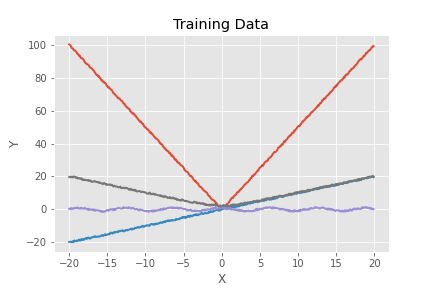
\includegraphics[width=12cm]{../output/figures/train.png}
\caption{Darstellung der bereitgestellten Trainingsdatensätze \cite{Gage:18}}\label{fig:train}
\end{figure}

Die Datei ideal.csv beinhaltet 50, nicht "verwaschene", idealtypische Funktionen in den Spalten "y1" bis "y50". Wie, im Detail im folgenden Unterkapitel beschrieben, sollen diese Funktionen durch das Programm mit dem Trainingsdatensatz verglichen werden und daraus die passendsten vier Funktionen gewählt werden. Die Datei weist, bis auf die Anzahl der Spalten, eine ähnliche Struktur wie der Trainingsdatensatz auf und besteht ebenfalls je Spalte aus 400 Datenpunkten. Auf die Darstellung eines exemplarischen Auszuges wird daher an dieser Stelle verzichtet.

%\begin{table}[H]
%\small
%\centering
%\csvreader[
%	tabular = |c|c|c|,
%	range={+5},
%	head to column names
%]{../data/ideal.csv}{}
%{}{\x & \y1 & \y50}
%\csvautotabular[range={+5}]{../data/ideal.csv}
%\caption{Exemplarischer Auszug der Datei ideal.csv}
%\label{tab:Exemplarischer Auszug aus ideal.csv}
%\end{table} 

Im Gegenzug zu den oben dargestellten beiden Datensätzen besteht der Testdatensatz nur aus 100 einzelnen Datenpunkten. Diese werden in einer Spalte "y" der Datei test.csv zusammengefasst und sind nicht als zusammengehörige Funktion zu verstehen. 

\begin{table}[H]
\small
\centering
\csvautotabular[range={+5}]{../data/test.csv}
\caption{Exemplarischer Auszug der Datei test.csv}
\label{tab:Exemplarischer Auszug aus test.csv}
\end{table} 

In der weiteren Bearbeitung der Aufgabenstellung sollen diese Datenpunkte mit den ausgewählten idealtypischen Funktionen verglichen und jeweils jener mit der geringsten Abweichung zugewiesen werden. Dieser Vorgang wird im Zuge dieser Arbeit als Klassifikation der Testdaten bezeichnet. Diese wird im Unterkapitel "Klassifikation der Testdaten" im Detail behandelt.

Gemäß der Vorgabe der Aufgabenstellung sollen sowohl die Trainings- (train.csv) als auch die Funktionsdaten (ideal.csv) in eine SQLite Datenbank eingelesen werden. Diese wird im Verzeichnis output/data bereitgestellt. Der Autor entschied sich hierbei für das Python-Modul sqlite anstelle des, in der Vorgabe vorgeschlagenen, Moduls sqlalchemy. Dieses bietet für die gegebene Anwendung eine vereinfachte Möglichkeit Daten mit einer SQLite Datenbank zu verarbeiten.

Über die UnitTests, die im Rahmen der, in Kapitel 1.2 beschriebenen, Modulinstallation durchgeführt werden, wird das lokale System auf die Möglichkeit eines direkten SQL-Imports hin überprüft. Dies bedeutet, dass versucht wird, die Daten in die SQLite Datenbank zu schreiben, ohne diese zuerst über das Python-Programm einzulesen und erst in einem weiteren Verarbeitungsschritt an die Datenbank übergeben zu müssen. Das Ergebnis der Überprüfung wird bei Erfolg im Logfile des Setups angeführt. 

Auch in der Ausführung des Programms wird vorerst noch einmal der direkte Import versucht und erst im Falle eines Fehlschlages der Umweg über die Funktionen des Python-Moduls pandas gewählt.

Obwohl, aufgrund der geringen Größe, der in dieser Arbeit vorliegenden Datendateien, die Möglichkeit des direkten Imports nur eine untergeordnete Rolle spielt, schont ein solcher im Falle von größeren Datenmengen die Systemressourcen und spart Zeit in der Programmausführung.

Die Testdaten (test.csv) werden, gemäß Vorgabe, in der Programmausführung zeilenweise eingelesen, mit den Daten der gewählten Funktionen verglichen und gemeinsam mit der getroffenen Klassifikation in die SQLite Datenbank geschrieben.

Für die interne Verarbeitung der Daten wurde, im Rahmen des Programms, eine eigene Objektklasse geschaffen, die spezifische Funktionen sowie die Parameter der Visualisierung bereitstellt. Diese Klasse und deren Unterklassen für die verschiedenen Datensätze sind in der Datei functionfinder/classes.py definiert.

\section{Auswahl idealtypischer Funktionen}

\begin{figure}[h]
\centering
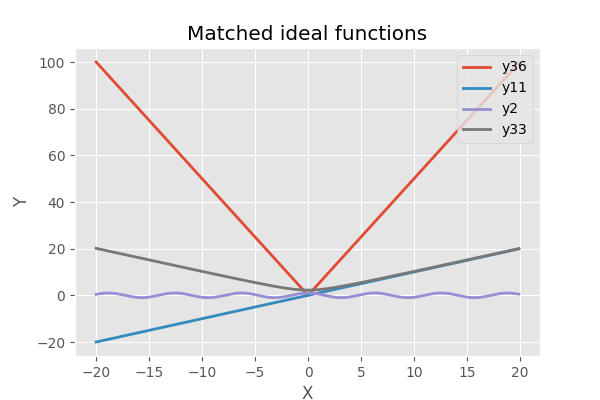
\includegraphics[width=12cm]{../output/figures/ideal.png}
\caption{Darstellung der ausgewählten idealtypischen Funktionen \cite{Gage:18}}\label{fig:ideal}
\end{figure}

\section{Klassifikation der Testdaten}

\begin{figure}[h]
\centering
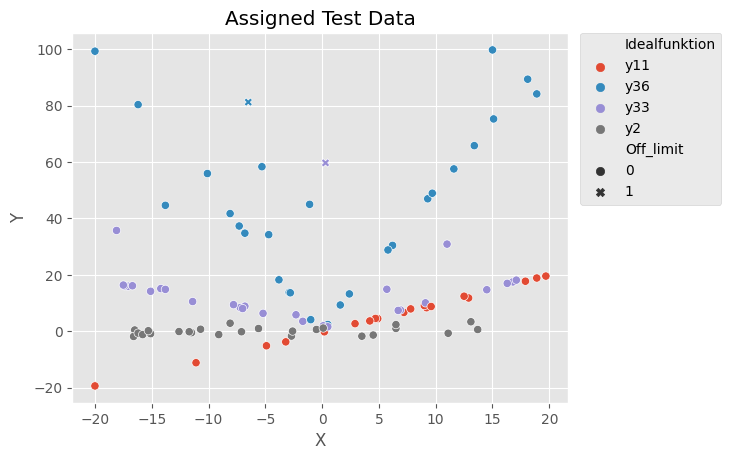
\includegraphics[width=12cm]{../output/figures/test.png}
\caption{Klassifikation der Testdatensätze \cite{Gage:18}}\label{fig:test}
\end{figure}


\chapter{Zusammenfassung}





% =========================================================
\section{Literature References}
Here is an example of a reference with a page-number: \cite[S. 6]{DueckKo:2016}


\section{Pictures}

\begin{figure}[h]
\centering

\includegraphics[width=8cm]{pics/spiral.pdf}
\caption{A spiral... smooth vector-based with a clean parametrisation! \\ Nothing to do with \cite{Gage:18}}\label{fig:spiral}
\end{figure}
\FloatBarrier

\section{Tables}

\begin{table}[H]
\small
\centering
\begin{tabular}{p{5cm}|l|p{3cm}}
`` Industrial era '' &  ``Jobs '' & `` Wanted: Upgrade''' \\ \hline
Parts exchanger & Fitter & mecatronics specialist \\
eShop & reseller & `` Client-suggester'' \\
`` Coding-guru''' & Softwaredesign & Whole-life designer \\
JA! Gut \& Günstig & brand-names & `` Life-Style Feeling'' \\
Internetbanking & Bank clerk & Customer adviser \\
Robots & Specialist & Machine supervisor \\
Bush & Gardener & Nature-sculptor \\
Painting & Painter & Interior Design \\
 &  & \\
\end{tabular}
\caption[Downgrade and upgrade of job denominations]{Downgrade and Upgrade of job denominations \\ \ \ \ \cite{DueckKo:2016}}
\label{tab:Downgrade and Upgrade of job denominations}
\end{table} 

\section{Listes}

\begin{itemize}
 \itemsep0pt
 \item one
 \item twoi
 \item threei
\end{itemize}

\begin{enumerate}
 \itemsep0pt
 \item first
 \item second
 \item third
\end{enumerate}


\section{Formulæ}

A formula can be written inline, e.g. as $ \frac{d}{dx}\mbox{arctg}(x) = \frac{1}{1+x^2}$ or, in centered math:

\begin{equation}  \frac{d}{dx}\mbox{arctg}(x) = \frac{1}{1+x^2} \label{arctanderivative}\end{equation}

Notice that formulæ that are centered start bigger (technically, they start in \verb+\displaystyle+) than they start inline (technically, they start in \verb+\textstyle+ all subsequents reductions, e.g. an exponent, goes to \verb+\scriptstyle+ then \verb+\scriptscriptstyle+). Indeed a best effort is made so that inline formulæ do not change the line height which would bother the eye of a reader.

Formulæ can be given a number and a label. Numbering happens automatically with \verb+\begin{equation}+ and \verb+\end{equation}+ and can be avoided if enclosing the formula betwee \verb+\[+ and \verb+\]+. If using the \verb+\label+ macro inside, you can refer automatically to this equation using \verb+\ref{label}+. E.g. Thanks to equation~\ref{arctanderivative} one dare say that:

\begin{equation} \int_0^t \frac{1}{1+x^2} dx = \mbox{arctan}(t) \end{equation}


\section{Tools and Code}

Many users of this template will want to include some code.

The simplest way to do so is to use the \verb+\verb+ macro which is followed by a sign, then some code, then the sign again to close. This is the inline version which works as in: 


\begin{verbatim}
As we could calculate with \cite{Wolfram_alpha} using 
\verb_integrate 1 / pi e ^ (t/pi) from zero to infinity_.
\end{verbatim}

which yields: 

As we could calculate with \cite{Wolfram_alpha} using \verb_integrate 1 / pi e ^ (t/pi)_ from zero to infinity.


The multiline version of this is called \verb+\begin{verbatim}+ and finishes with \verb+\end{verbatim}+.


\section{Citation examples}

Monography \citep[][S. 22]{con:infra} 

Collection \citep{sammelband} 

Article \citep{article1}
